\documentclass{beamer}

\usepackage{graphicx}
\usepackage{tikz}
\usepackage{lmodern}
\usepackage{mathtools}

\usetheme{CambridgeUS}
\usecolortheme{beaver}
\setbeamercovered{transparent}
\usefonttheme{professionalfonts}
\setbeamertemplate{itemize items}[default]

\begin{document}

\title[Compact finite differences on GPUs]
{A novel approach to evaluating 
compact finite differences 
and similar tridiagonal schemes on GPU-accelerated clusters}

\author[Ashwin Srinath]{
        Ashwin Srinath\\
        Department of Mechanical Engineering\\
        \today}
\date{}
\titlepage

\begin{frame}{Overview}
    \tableofcontents
\end{frame}

\section{Introduction}
\begin{frame}
\frametitle{Motivation}
\begin{itemize}[<+->]
    \item Computation established as the ``third way''
        to scientific truth
    \item Solving real problems:
        energy research,
        climate modeling,
        protein folding,
        quantum mechanics...
    \item Computational power soon becomes the bottleneck
        for the size and scope of the problems that can
        be solved
    \item Computational science and
        \emph{high-performance computing} have become
        synonymous
\end{itemize}
\end{frame}

\begin{frame}
\frametitle{Graphics processing units}
\begin{columns}[c]
     \begin{column}[T]{5cm}
        Expectations
        \begin{figure}
        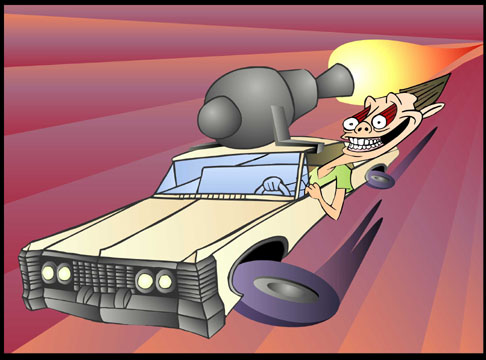
\includegraphics[width=150px]{img/expectations.jpg}
        \end{figure}
    \end{column}

    \begin{column}[T]{5cm}
        Reality
        \begin{figure}
        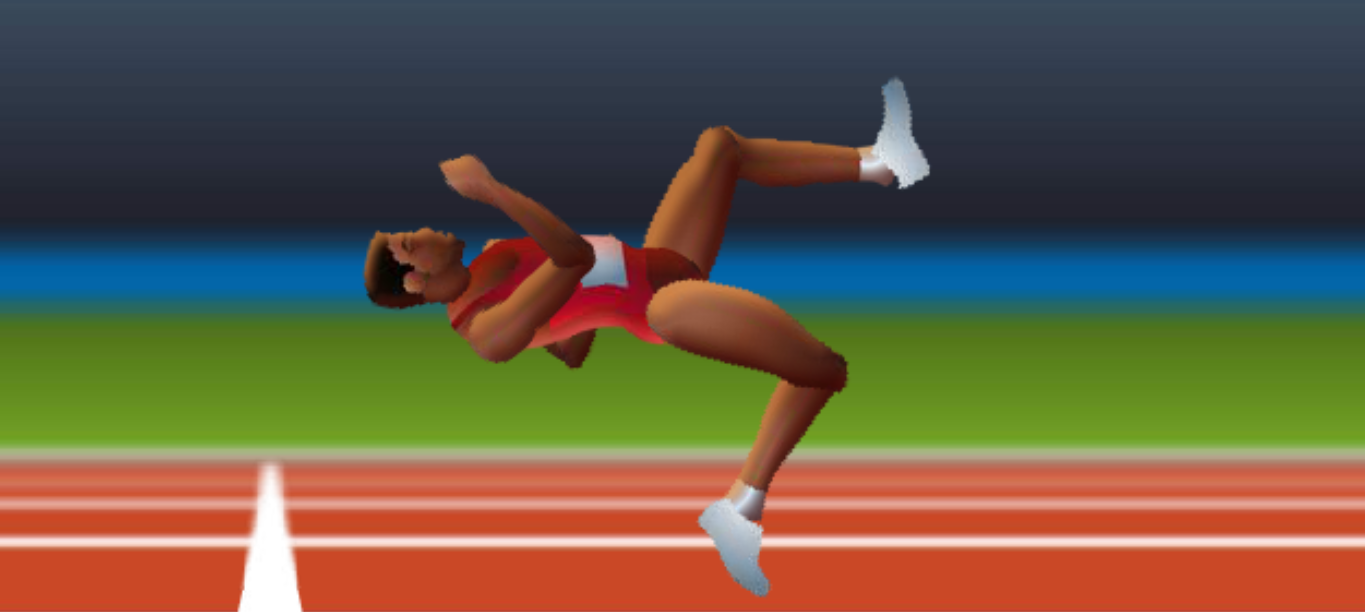
\includegraphics[width=150px]{img/reality.png}
        \end{figure}
    \end{column}
\end{columns}
\end{frame}

\section{Proposed Tridiagonal Algorithm}
\section{Distributed Compact Finite Difference Evaluation}
\section{Results}

\end{document}
